\documentclass[tikz,border=2pt]{standalone}
\usepackage{fontspec}
\setmainfont{texgyretermes-regular.otf}
\usepackage{pgfplots}
\pgfplotsset{compat=1.18}
\begin{document}
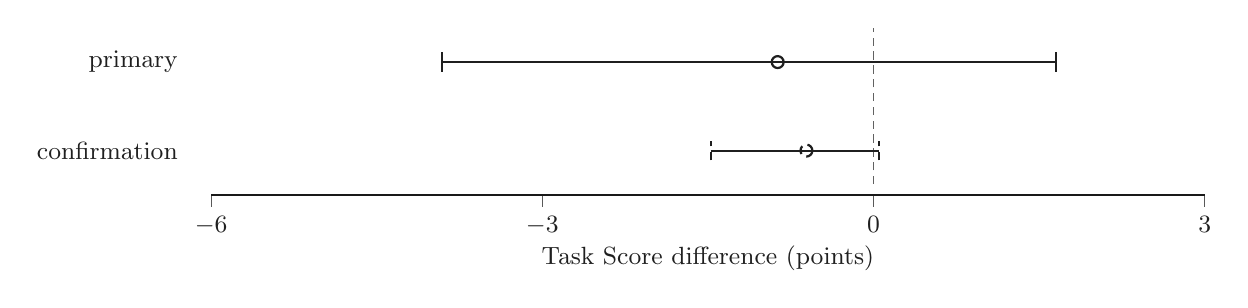
\begin{tikzpicture}
\begin{axis}[
  width=14.2cm,height=3.83cm,
  xmin=-6,xmax=3,ymin=-0.5,ymax=1.5,
  xtick={-6,-3,0,3},
  ytick={},yticklabels={},
  xlabel={Task Score difference (points)},
  axis x line*=bottom,axis y line=none,
  tick align=outside,
  tick style={line width=0.35pt,color=black!65},
  axis line style={line width=0.55pt,color=black!90},
  tick label style={font=\small,color=black!88},
  yticklabel style={font=\small,color=black!88},
  label style={font=\small,color=black!88},
  xlabel style={yshift=1mm},
  yticklabel shift=1mm,
  grid=none,clip=false,
]
\draw[densely dashed,line width=.55pt,color=black!62] (axis cs:0,-0.38) -- (axis cs:0,1.38);
\addplot+[no markers,color=black!88,line width=.7pt] coordinates {(-3.90625,1)(1.64930555555556,1)};
\addplot+[only marks,mark=o,mark size=2.15pt,mark options={color=black!88,fill=white,line width=.8pt}] coordinates {(-0.868055555555555,1)};
\addplot+[no marks,color=black!88,line width=.7pt] coordinates {(-3.90625,0.89)(-3.90625,1.11)};
\addplot+[no marks,color=black!88,line width=.7pt] coordinates {(1.64930555555556,0.89)(1.64930555555556,1.11)};
\addplot+[no markers,color=black!88,line width=.7pt] coordinates {(-1.47569444444445,0)(0.0520833333333333,0)};
\addplot+[only marks,mark=o,mark size=2.15pt,mark options={color=black!88,fill=white,line width=.8pt}] coordinates {(-0.607638888888889,0)};
\addplot+[no marks,color=black!88,line width=.7pt] coordinates {(-1.47569444444445,-0.11)(-1.47569444444445,0.11)};
\addplot+[no marks,color=black!88,line width=.7pt] coordinates {(0.0520833333333333,-0.11)(0.0520833333333333,0.11)};
\node[anchor=east,font=\small,text=black!88] at ([xshift=-3mm]axis cs:-6,1) {primary};
\node[anchor=east,font=\small,text=black!88] at ([xshift=-3mm]axis cs:-6,0) {confirmation};
\end{axis}
\end{tikzpicture}
\end{document}
